\section{Security Context}
\label{sec:securitycontext}

\begin{figure}
    \centering
        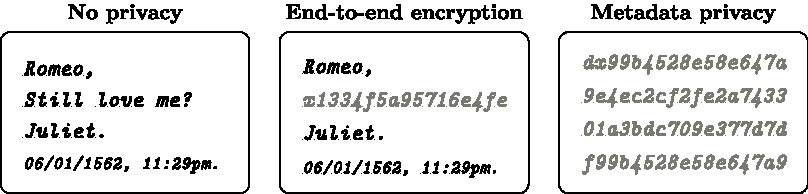
\includegraphics[width=\textwidth]{metadata-privacy.pdf}
\caption{The view of a powerful adversary in three different threat models. With end-to-end encryption, the adversary can still see the metadata.}
\label{fig:metadataprivacy}
\end{figure}



In this section, we describe what our system achieves beyond end-to-end encrypted messaging applications like Signal and Wickr.

Signal is great. It is end-to-end encrypted, open source, and run by a trustworthy group. Unfortunately, if their servers are hacked, one of their employees bribed, or you are attacked by a network-level powerful actor, there is nothing Signal can guarantee. \xxx[stzh]{I do not think so. The point of E2E encryption is to guarantee content security when the server gets compromised.}

Furthermore, even with a secure server, it leaks metadata.  Using timing attacks, an adversary can figure out when, where and with whom you are talking. 

\subsection{Desired Properties}

1. \textbf{Metadata Protection}: All contents and metadata of a conversation are only visible to the users involved in the conversation. Even with all servers compromised, an adversary should not be able to find out whether two users are engaging in conversation.

An especially challenging case is metadata protection during trust establishment. This happens when two users wish to add each other as friends for the first time. This feature is not supported even by Addra or Pung. We outline our solution in \cref{sec:trustestablishment}, which offers users a variety of options to establishing trust.

2. \textbf{Resistance to MITM attacks}: We use PIR and end-to-end encryption to ensure no man-in-the-middle(MITM) can access metadata associated with any conversation of the user.

3. \textbf{Resistance to DoS attacks}: Denial of Service(DoS) attacks are unavoidable if the adversary controls all our servers. In the case of a server-controlling adversary, we do not guarantee liveliness of our service, but continue to guarantee metadata security. We also defend against DoS attacks launched by an end-user with no access to the servers.

4. \textbf{Reasonable Load on Client and Server}: Since PIR is expensive, we design our system to minimize load on the client and server without compromising security. We use the most efficient PIR algorithms known on the server. We also give users the option to adjust client side load to suit their upload and download bandwidth.

\section{Threat Model}

\todo{add table comparing our threat model with e.g. signal and email}
\todo{add an illustration of a walled garden, with the walls containing only your computer and your friends' computers}

%Touch on: server, friends, client-side computer, etc.

\todo{Figure out a better format here. See e.g. Skiff's whitepaper.}



Similar to most PIR schemes(for example \cite{ahmad2021addra}, \textsection 2.2), our threat model assumes a global adversary who can compromise the entire communication infrastructure except for the user's and their friends' client end. In particular, we assume the adversary has control over all the servers, and can observe and manipulate all network traffic.

End-user trust is more subtle matter. In \cite{angel2018s}, Angle, Lazar and Tzialla describes the compromised friend(CF) attack on a general meta-data private messaging system, which shows that perfectly hiding metadata while not trusting the user's friends is computationally prohibitive. In our security model, a user trusts that the devices of themselves and all their friends are uncompromised and running an unmodified copy of anysphere's client-side code. The user assumes that any other end-user device might be compromised.

\todo{Can we assume that only a small number of friends are compromised?}

Finally, we assume the security of the standard cryptography primitives we use, including microsoft SEAL's BFV cryptosystem and libsodium's AEAD cryptosystem. 

Denial of Service(DoS) attacks are unavoidable if the adversary controls all our servers. In the case of such attacks, we do not guarantee liveliness of our service, but continue to guarantee metadata security. We also defend against DoS attacks launched by an end-user with no access to the servers.

\subsection{Desired Properties}

1. \textbf{Perfect Metadata Protection}: All contents and metadatas associated with a conversation are only visible to the users involved with the conversation. Even with a compromised server, an adversary should not even be able to find out whether two users are engaging in any conversation.

2. \textbf{Forward Secrecy}: \todo{do we provide this?}

3. \textbf{Resistant to man-in-the-middle attacks}.

4. \textbf{Resistant to social engineering attacks}.

\todo{add more.}



